\documentclass[12pt]{article}

% DEFAULT PACKAGE SETUP
\usepackage{setspace,graphicx,epstopdf,amsmath,amsfonts,amssymb,amsthm,geometry}
\usepackage{marginnote,datetime,enumitem,rotating,fancyvrb}
\usepackage{threeparttable,float,soul,booktabs}
\usdate
\geometry{scale=0.8}

% FONT
\usepackage{xeCJK,fontspec} 
\setCJKmainfont{KaiTi}
\setCJKmonofont{SimSun} 
%\usepackage{newtxtext,newtxmath} % Times New Roman
%\usepackage{newpxtext,newpxmath} % Too Slim
%\usepackage{fouriernc} 		  % Too Curved
\usepackage{fourier}    		  % Favourite Font

%% Use natbib.sty.
\usepackage{natbib,fancybox,url,graphicx,color}
\definecolor{MyBlue}{rgb}{0,0.2,0.6}
\definecolor{MyRed}{rgb}{0.4,0,0.1}
\definecolor{MyGreen}{rgb}{0,0.4,0}
\usepackage[bookmarks=true,bookmarksnumbered=true,colorlinks=true,linkcolor=MyBlue,citecolor=MyRed,filecolor=MyBlue,urlcolor=MyGreen]{hyperref}

\usdate
\geometry{scale=0.8}

%% Use natbib.sty.
\usepackage{natbib,fancybox,url,graphicx,color}
\definecolor{MyBlue}{rgb}{0,0.2,0.6}
\definecolor{MyRed}{rgb}{0.4,0,0.1}
\definecolor{MyGreen}{rgb}{0,0.4,0}
\usepackage[bookmarks=true,bookmarksnumbered=true,colorlinks=true,linkcolor=MyBlue,citecolor=MyRed,filecolor=MyBlue,urlcolor=MyGreen]{hyperref}
\bibliographystyle{aer}

%% Theorem Environment
\theoremstyle{definition}
\newtheorem{theorem}{Theorem}
\newtheorem{acknowledgement}[theorem]{Acknowledgement}
\newtheorem{algorithm}[theorem]{Algorithm}
\newtheorem{axiom}[theorem]{Axiom}
\newtheorem{case}[theorem]{Case}
\newtheorem{claim}[theorem]{Claim}
\newtheorem{conclusion}[theorem]{Conclusion}
\newtheorem{condition}[theorem]{Condition}
\newtheorem{conjecture}[theorem]{Conjecture}
\newtheorem{corollary}[theorem]{Corollary}
\newtheorem{criterion}[theorem]{Criterion}
\newtheorem{definition}{Definition} % Number definitions on their own
\newtheorem{derivation}{Derivation} % Number derivations on their own
\newtheorem{example}[theorem]{Example}
\newtheorem{exercise}[theorem]{Exercise}
\newtheorem{lemma}[theorem]{Lemma}
\newtheorem{notation}[theorem]{Notation}
\newtheorem{problem}[theorem]{Problem}
\newtheorem{proposition}{Proposition} % Number propositions on their own
\newtheorem{remark}[theorem]{Remark}
\newtheorem{solution}[theorem]{Solution}
\newtheorem{summary}[theorem]{Summary}
\newtheorem{assumption}[theorem]{Assumption}

\begin{document}
\title{\bf {Uninsured Idiosyncratic Risk and Aggregate Saving - QJE - 1994}}
\author{Wenzhi Wang \thanks{This note is written down during my M.phil. period at the University of Oxford. } }
\date{\today}

\maketitle

\section{Economics with Heterogeneous Agents, Uninsured Idiosyncratic Shocks, and Borrowing Constraints: An Exposition}


\subsection{The Individual's Problem}
Let $U(c)$ be the period utility function, $\beta$ be the utility discount factor with $\lambda = \frac{1}{\beta} -1$ being the time preference rate. Assume that labor endowment shocks (equivalently, earnings) are iid over time. We also permit some borrowing. The individual's problem is to maximize
\begin{equation}
	\label{1a} \tag{1a}
	\operatorname{E}_0 \left\{\sum_{t=0}^\infty \beta^t U(c_t) \right\}
\end{equation}
subject to
\begin{equation}
	\label{1b} \tag{1b}
	c_t + a_{t+1} = w l_t + (1+r) a_t; \; c_t \geq 0, \; a_t \geq -b, 
\end{equation}
where $b$ (if positive) is the limit on borrowing and $l_t$ is assumed to be iid with bounded support given by $\left[l_{\min}, l_{\max} \right]$, with $l_{\min} > 0$.

Clearly, if $r<0$, some limit on borrowing is required. Otherwise, the problem is not well posed, and a maximum does not exist. The present value of earnings is infinite and nothing prevents the individual from running a Ponzi scheme. If $r>0$, then a less restrictive alternative to imposing a borrowing limit is to impost present value budget balance. This is equivalent to requiring $\lim
_{t\rightarrow \infty} \frac{a_t}{(1+r)^t} \geq 0$. In turn, the limit condition together with the non-negativity of consumption is equivalent to the period-by-period borrowing constraint $a_t \geq \frac{-w l_{\min}}{r}$. Thus, \emph{a borrowing constraint is necessarily implied by non-negative consumption}. Further, if $b$ exceeds $w l_{\min} /r$, then the borrowing limit will never be binding, and $b$ may be replaced by the smaller amount $w l_{\min} /r$. Therefore, without loss of generality we may specify the limit on borrowing as 
\begin{equation}
	\label{2a} \tag{2a}
	a_t \geq -\phi
\end{equation}
\begin{equation}
	\label{2b} \tag{2b}
	\phi \equiv \min \left\{b, \frac{w l_{\min}}{r} \right\}, \text{ for } r>0;\; \phi \equiv b, \text{ for } r<0
\end{equation}

If the borrowing limit $b$ is tighter than $wl_{\min}/r$ (e.g., if $b$ is zero so that no borrowing is permitted), then the borrowing limit $b$ may be regarded as ad hoc in the sense that it is not a consequence of present value budget balance and non-negativity of consumption. Note that $\phi$ is to be regarded as a function of $b$, $w$, and $r$. Equation \ref{2a} will be referred to as a ``fixed'' borrowing limit. 

We now define $\hat{a}_t$ and $z_t$ as follows:
\begin{equation}
	\label{3a} \tag{3a}
	\hat{a}_t = a_t + \phi
\end{equation}
\begin{equation}
	\label{3b} \tag{3b}
	z_t = w l_t + (1+r) \hat{a}_t - r\phi,
\end{equation}
where $z_t$ may be thought of as the total resources of the agent at date $t$. Now we can rewrite \ref{1b} as follows:
\begin{equation}
	\label{4a} \tag{4a}
	c_t + \hat{a}_{t+1} = z_t, \; c_t \geq 0, \; \hat{a}_t \geq 0,
\end{equation}
\begin{equation}
	\label{4b} \tag{4b}
	z_{t+1} = w l_{t+1} + (1+r) \hat{a}_{t+1} - r\phi.
\end{equation}

Let $V(z_t, b, w, r)$ be the optimal value function for the agent with total resources $z_t$. This function is the unique solution to the following Bellman's equation:
\begin{equation}
	\label{5} \tag{5}
	V\left(z_t, b, w, r\right) \equiv \max_{\hat{a}_{t+1}} \left\{U\left(z_t-\hat{a}_{t+1}\right)+\beta \int V\left(z_{t+1}, b, w, r\right) d F\left(l_{t+1}\right)\right\},
\end{equation}
where the maximization on the right side is over $\hat{a}_{t+1}$ subject to (\ref{4a}) and (\ref{4b}).

The optimal asset demand function is 
\begin{equation}
	\label{6} \tag{6}
	\hat{a}_{t+1} = A(z_t, b, w, r).
\end{equation}

Substituting (\ref{6}) into (\ref{4b}), we obtain the transition law for total resources $z_t$:
\begin{equation}
	\label{7} \tag{7}
	z_{t+1} = w l_{t+1} + (1+r)A(z_t, b, w, r) - r\phi.
\end{equation}

In Figures \ref{figIa} and \ref{figIb} we show some typical shapes for the functions on the right sides of (\ref{6}) and (\ref{7}), \emph{\bf under the assumption that the interest rate $r$ is less than the rate of time preference $\lambda$}. Clearly, the agent would like to borrow but is limited by the borrowing limit. As total resources get smaller and smaller, the individual borrows more and more in order to maintain current consumption, and his debt approaches the borrowing limit. At some point when total resources are too low, it would be optimal to borrow up to the limit and consume all the total resources. Thus, there exists a positive value $\hat{z} > z_{\min} \equiv wl_{\min} - r\phi \geq 0$, such that whenever $z_t \leq \hat{z}$, it is optimal to consume all the total resources, i.e., set $c_t = z_t$ and set $\hat{a}_{t+1}$ to its lowest permissible value, which is zero. For $z_t \geq \hat{z}$, both $c_t$ and $\hat{a}_{t+1}$ are strictly increasing in $z_t$; i.e., $A(\cdot)$ is strictly increasing with a slope less than 1. In this situation, the borrowing limit is not currently binding.

Under some additional assumptions, the support of the Markov process defined by (\ref{7}) is bounded; specifically there is a $z^*$ such that for all $z_t \geq z^*, z_{t+1} \leq z_t$ with probability one. These conditions also guarantee that there exists a unique, stable stationary distribution for $\{z_t\}$ which behaves continuously with respect to the parameters $b, w$ and $r$. Let $Ea_w$ (the subscript reflecting the fact that for now $w$ is being treated as fixed) denote long-run average assets. Using (\ref{3a}) and (\ref{6}), this is given by 
\begin{equation}
	\label{8} \tag{8}
	Ea_w = E \left[A(z, b, w, r)\right] - \phi,
\end{equation}
where $E[\cdot]$ denotes the expectation with respect to the stationary distribution of $z$.

\subsection{Endogenous Heterogeneity and Aggregation}

\begin{figure}
	\centering
	\begin{minipage}{.5\linewidth}
		\caption{}	
		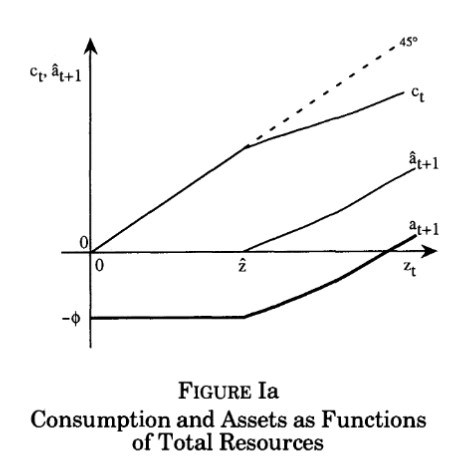
\includegraphics{figIa.jpg}
		\label{figIa} 
		
	\end{minipage}
	\begin{minipage}{.45\linewidth}
		\caption{}
		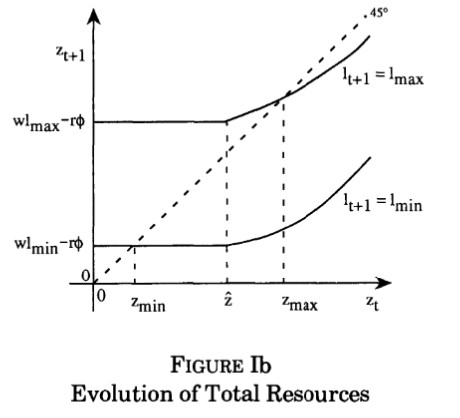
\includegraphics{figIb.jpg}
		\label{figIb}
		
	\end{minipage}
\end{figure}

\begin{figure}
	\centering
	\begin{minipage}{.5\linewidth}
		\caption{}
		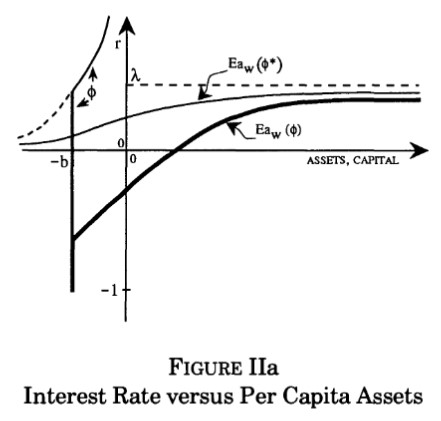
\includegraphics{figIIa.jpg}
		\label{figIIa}
		
	\end{minipage}
	\begin{minipage}{.45\linewidth}
		\caption{}
		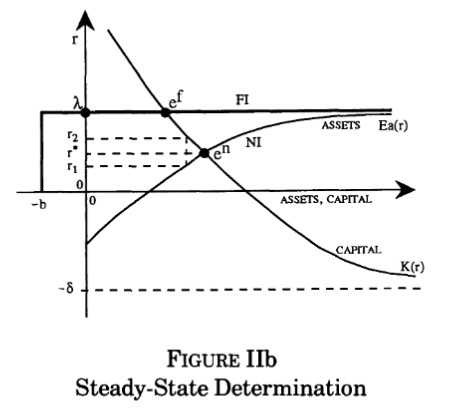
\includegraphics{figIIb.jpg}
		\label{figIIb}
		
	\end{minipage}
\end{figure}

The distribution of $\{z_t\}$ and the value of $Ea_w$ reflect the endogenous heterogeneity and the aggregation features. $Ea_w$ represents the aggregate assets of the population consistent with the distribution of assets across the population implied by individual optimal saving behavior. In Figure \ref{figIIa} we show a typical shape of the graph of $Ea_w$ versus $r$.

The most important feature of this graph is that $Ea_w$ tends to infinity as $r$ approaches the rate of time preference $\lambda$ from below. This reflects the infinite horizon of consumers. \emph{If $r$ equals or exceeds the rate of time preference, then the individual will accumulate an infinitely large amount of assets, and $Ea_w$ may be thought to be infinity.} Intuitively, if $r$ exceeds $\lambda$, then the individual wants to postpone consumption to the future and be a lender. The consumption profile will be upward sloping, and the agent will accumulate an infinitely large amount of assets to finance an infinitely large amount of consumption in the distant future. 

This conclusion carries over to the borderline case of $r$ equal to $\lambda$. In this case, the consumer attempts to maintain a smooth marginal utility of consumption profile. At the margin it is costless for the consumer to acquire an additional unit of the asset. However, since there is a positive probability of getting a sufficiently long string of bad draws of labor shocks, maintaining a smooth marginal utility of consumption profile is only possible if the consumer has an arbitrarily large amount of assets to buffer the shocks.

Next, note that \emph{\bf for values of $r < \lambda$, $Ea_w$ is always higher under uncertainty than if earnings were certain, at least so long as $r$ is not too much below $\lambda$; i.e., assets are not too costly to hold. This result is independent of whether $U^{\prime}$ is convex or concave and arises due to the borrowing constraint and the infinite horizon.} In a single consumer problem with a two-period horizon, there is no heterogeneity, and the borrowing constraint may be ignored by making suitable assumptions about the time profile of earnings. However, with an infinite horizon, repeated shocks, and $r < \lambda$, neither the heterogeneity nor the borrowing constraint can be ignored.

If earnings were certain (or, equivalently, markets complete), $Ea_w$ would equal $-\phi$ for all $r < \lambda$. That is, per capita assets under certainty are at their lowest permissible level since all agents are alike and everyone is constrained. However, in a steady state under incomplete markets, there is a distribution of agents with different total resources reflecting different histories of labor endowment shocks. Those with low total resources will continue to be liquidity constrained, whereas those with high total resources will accumulate assets beyond the constrained level regardless of the convexity of marginal utility simply because their current total resources are quite high relative to average future total resources. Aggregation then implies that per capita assets must necessarily exceed their level under certainty.

\subsection{General Equilibrium}

The crucial features that explain how uninsured idiosyncratic shocks and borrowing constraints lead to higher aggregate saving are that $Ea_w$ is finite only if $r$ is less than $\lambda$ and that it tends to infinity as $r$ approaches $\lambda$ from below. To see this, let $f(k, 1)$ denote per capita output as a function of per capita capital $k$ and per capita labor (which equals unity), and let $\delta$ be the depreciation rate of capital. Now consider the curve labeled $K(r)$ in Figure (\ref{figIIb}). Under standard assumptions, this curve is downward sloping, tends to $\infty$ as r tends to $-\delta$, and tends to zero as r tends to $\infty$. In addition, we can express the wage $w$ as a function of $r$ since $w$ equals $f_2(k, 1)$. Denote this by $\omega(r)$, which is a decreasing function under standard assumptions, tends to zero as $r$ tends to $\infty$, and tends to $\infty$ as $r$ tends to $-\delta$. For a given $r$, let $Ea$ denote the value of $Ea_w$ when $w$ equals $\omega(r)$, and let NI (for no insurance) be the graph of $Ea(r)$ versus $r$. A steady state of this economy is then characterized by the condition $K(r) = Ea(r)$. Intuitively, one may think of $K(r)$ as the capital desired by firms at the interest rate r, and $Ea(r)$ as the capital supplied by households at the interest rate r.

Now consider what the steady state of the economy would be if there were no uncertainty, or, equivalently, there were full insurance markets. Then the economy consists of a representative agent who receives the constant earnins $w$ in each period. \emph{\bf If $r$ is less than $\lambda$, the agent would always be up against his borrowing limit, and his asset holdings would be $-\phi$. If $r$ equals $\lambda$, his asset holdings equal his initial holdings whatever they may be. If $r$ exceeds $\lambda$, then he would accumulate an infinitely large amount of assets.} Therefore, the right-angled line labeled FI (for full insurance) consisting of the horizontal segment at the height $\lambda$ and the vertical segment corresponding to the binding borrowing constraint represents the individual's desired asset holdings as a function of $r$. The steady state of his full insurance economy is at the point $e^f$.

It is clear from the proceeding argument that the aggregate capital stock is higher and the interest rate is lower in the economy with uninsured idiosyncratic shocks and borrowing constraints as compared with the standard economy. The saving rate, which is given by $\delta k / f(k, 1)$ is also higher.

The above analysis also explains why general equilibrium considerations in combination with the shape of the $Ea(r)$ curve can play an important role in limiting the impact of idiosyncratic risk and liquidity constraints on aggregate saving. Since $Ea$ approaches infinity as $r$ approaches $\lambda$ from below, average household assets are extremely sensitive to slight variations in the interest rate when it is close to (but below) the rate of time preference. In a partial equilibrium analysis, by choosing an interest rate close enough to the rate of time preference, one can generate arbitrarily large precautionary saving in excess of the certainty case. However, in general equilibrium $r$ is determined endogenously and how much $r$ is reduced relative to the certainty case, thereby, how much aggregate saving is increased is then a quantitative issue.

We shall briefly describe the effects of varying the borrowing limit $b$. This is related to two other features of the $Ea_w$, curve in Figure (\ref{figIIa}). When $r$ equals negative unity (so that the gross return on assets is zero), assets will always equal ($-b$). When $r$ equals zero, $b$ is not an argument of the asset demand function $A ( )$. Hence, $Ea_w$, decreases one-to-one with increases in $b$ when $r$ is zero. These two features suggest that the $Ea_w$, curve shifts to the left when $b$ increases. Therefore, permitting a higher borrowing limit serves to lower aggregate capital and raise the interest rate toward the time preference rate Figure (\ref{figIIb}). The intuition behind this conclusion is that when borrowing is permitted individuals need not rely solely on holdings of capital to buffer earnings variation. Borrowing can also be used to buffer these shocks and, hence, leads to smaller holdings of capital.

It follows from the previous remarks that if uninsured idiosyncratic risk and no borrowing $(b = 0)$ lead to a small increase in aggregate capital relative to the certainty case, then permitting some borrowing $(b > 0)$ will lead to an even smaller increase in aggregate capital.

We briefly describe the effects of setting $a_t \geq -\phi^* \equiv w l_{\min}/r$ and restricting $r$ to be positive. As noted earlier, this is the appropriate form of the borrowing constraint implied by present value budget balance and non-negativity of consumption when $r>0$, and will be referred to as the ``present value'' borrowing constraint. If $l_{\min}$ is zero, this is equivalent to the case of no borrowing ($b=0$). However, if $l_{\min}$ is positive, then $Ea_w$ tends to $-\infty$ as $r$ tends to zero (see Figure \ref{figIIa}, the curve marked $Ea_w(\phi^*)$). This can be seen by substituting $wl_{\min}$ for $\phi$ in equations (\ref{3a})-(\ref{8}). The first term on the right side of (\ref{8}) remains finite, whereas the second term tends to $-\infty$ as $r$ tends to zero. Intuitively, as $r$ becomes smaller, the borrowing limit becomes larger, permitting the individual to carry large amounts of debt. That is, the present value of minimum earnings is tending to infinity, enabling the individual to service large amounts of debt. The main difference between this case and the case of a fixed borrowing limit is that under the present value borrowing constraint there always exists a steady state with a positive interest rate. With a fixed borrowing limit there may be no steady state with a positive interest rate though there does exist a steady state with a negative interest rate.

\subsection{Some Alternative Interpretations}

The model of individual optimization in (\ref{1a},\ref{1b}) can be turned into a pure exchange model with government debt in order to analyze the effects of changing the level of government debt. Let the government have outstanding a constant per capita amount of debt denoted by $d$, the interest on which is financed by an equal (across agents) lump sum tax $\tau = rd$. Then the consumer's budget constraint (\ref{1b}) is altered to $c_t + a_{t+1} = wl_t - rd + (1+r)a_t$. The steady-state equilibrium condition is $Ea_w = d$, where $Ea_w$ denotes per capita asset holdings in the steady state.

In this model whether debt neutrality holds or not depends crucially on how the borrowing constraint is specified. With a fixed borrowing limit as in (\ref{2a}, \ref{2b}), debt neutrality will not hold. However, with a present value borrowing constraint, i.e., when the borrowing limit equals the present value of minimum earnings adjusted for tax obligations, so that we have $a_t \geq -(wl_{\min}-rd)/r$, then debt neutrality does hold. The equilibrium interest rate, the distribution of asset holdings net of government debt, and consumption are invariant to the level of d. This can be seen by using the transformation $a^{*} = a_t - d$ in the above equations. Thus, the validity of debt neutrality in this framework with incomplete markets is entirely dependent on whether the borrowing limit takes account of changing tax obligations.

The model of individual optimization in (\ref{1a},\ref{1b}) can also be turned into an "optimum quantity of money" model as in Bewley [1983].

\section{Model Specification, Parameterization, and Computation}

The model period is taken to be one year, and the utility discount factor $\beta$ is chosen to be 0.96. The production function $f$ is assumed to be Cobb-Douglas with the capital share parameter (denoted $\alpha$) taken to be 0.36. The depreciation rate of capital ($\delta$) is set at 0.08. The period utility function is of the constant relative risk aversion (CRRA) type, with $\mu$, the relative risk aversion coefficient is set to be $\{1, 3, 5\}$.

For the labor endowment shocks we use a Markov chain specification with seven states to match the following first-order autoregressive representation for the logarithm of the labor endowment shock (equivalently, earnings):
\begin{equation}\label{9} \tag{9}
	\log \left(l_t\right)=\rho \log \left(l_{t-1}\right)+\sigma\left(1-\rho^2\right)^{1 / 2} \epsilon_t, \epsilon_t\sim\operatorname{Normal}(0,1),
\end{equation}
\begin{equation}\label{10} \tag{10}
	\sigma \in\{0.2,0.4\}, \rho \in\{0,0.3,0.6,0.9\}.
\end{equation}

The coefficient of variation equals $\sigma$ and the serial correlation coefficient equals $\rho$. We then follow the standard procedure to approximate the above autoregression by a seven-state Markov chain.

Note that we have made no allowance for the possibility that reported earnings variabilities contain significant measurement error. However, this is a serious possibility, and the relevant degree of idiosyncratic earnings variability may be somewhat lower. However, this is balanced by the possibilities that the data do not include uninsured losses and taste shocks.

Last, the borrowing limit $b$ is set to zero; i.e., borrowing is prohibited. As explained in the previous section, permitting some borrowing would lead to even smaller effects on the aggregate saving rate.

\subsection{Computation}

We approximate the asset demand as a function of total resources (for each of seven possible current labor endowment shocks) by a continuous, piece-wise linear function over an interval. The corresponding partition of the interval is chosen to be finer at the lower end of the interval and coarser at the upper end of the interval\footnote{The reason is that for low levels of total resources assets will be zero since the borrowing constraint will bind. At some critical level of total resources, assets will become positive. This introduces a high degree of nonlinearity into the asset demand function. Consequently, it is important to have a finer partition at the lower end of the interval to obtain a good approximation. It turned out that throughout the upper half of the interval the asset demand function was very nearly linear so that a coarse partition was adequate to obtain a good approximation in this region.}. 

The algorithm for approximating the steady state uses simulated series and the bisection method. We start with some value of $r$ (say, $r_1$) close to but less than the rate of time preference (see Figure (\ref{figIIb})). 
We then compute the asset demand function as described above. We then simulate the Markov chain for the labor endowment shock using a random number generator and obtain a series of 10000 draws. These are used with the asset demand function to obtain a simulated series of assets. The sample mean of this is taken to be $Ea$. 
We then calculate $r_2$ such that $K(r_2)$ equals $E(a)$. If $r_2$ exceeds the rate of time preference, it is replaced by the rate of time preference. Now note that by construction $r_1$ and $r_2$ are on opposite sides of the steady-state interest rate $r^*$. Without loss of generality, we may suppose that $r_1<r^*<r_2$. We then define $r_3 = (r_1 + r_2)$ and calculate $Ea$ corresponding to $r_3$. If $Ea$ exceeds $K(r_3)$, then $r_2$ is replaced by $r_3$, and we use bisection again. If $Ea$ is less than $K(r_3)$, then $r_1$ is replaced by $r_3$, and we use bisection again. Typically, this yields an excellent approximation to the steady state within ten iterations.

Once the steady state is approximated, we use the solution to calculate the following objects of interest. We calculate the mean, median, standard deviation, coefficient of variation, skewness, and serial correlation coefficient for labor income, asset (capital) holdings, net income, gross income, gross saving, and consumption. These descriptive statistics are based on the simulated series obtained in the manner described before.

\end{document}